\documentclass{article}
\usepackage[utf8]{inputenc}
\usepackage{parskip}
\usepackage{graphicx}
\usepackage{float}

\title{Lab3 Machine Learning}
\author{Casper Renman\\casperr@kth.se \and Hampus Fristedt\\hamfri@kth.se}
\begin{document}
\maketitle

\section{Assignment 3} 

\subsection{Does the feature independence assumption have any effect on the
classification accuracy for the different datasets?} 
Yes. The worst effect of assuming feature independence is on the vowel dataset.

\subsection{If so why does some of the datasets have more difference than
others?}

Because some datasets features are more dependent than others.

\subsection{When can an independence assumption be reasonable and when not?}

If the features of a datasets are losely correlated, an independence assumption 
is reasonable.

\subsection{How does the standard deviation differ for the two assumptions and
what does that imply?}

If we assume feature independence, the standard deviation is bigger.

% \subsection{Polynomial}
% \begin{figure}[H]
%     \centering
%     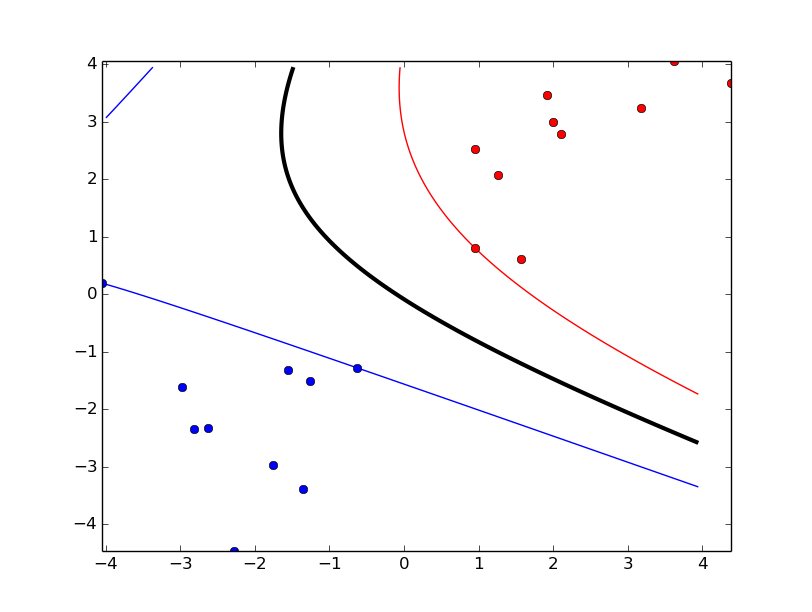
\includegraphics[width=1.0\linewidth]{../img/poly_s1_ez_p2.png}
% \end{figure}

\end{document}
